\section {Текст задания}
Для выполнения лабораторной работы №1 необходимо:
\begin{itemize}

	\item На основе предложенной предметной области (текста) составить ее описание. Из полученного описания выделить сущности, их атрибуты и связи.
	\item Составить инфологическую модель.
	\item Составить даталогическую модель. При описании типов данных для атрибутов должны использоваться типы из СУБД PostgreSQL.
	\item Реализовать даталогическую модель в PostgreSQL. При описании и реализации даталогической модели должны учитываться ограничения целостности, которые характерны для полученной предметной области.
	\item Заполнить созданные таблицы тестовыми данными. 
\end{itemize}
Для создания объектов базы данных у каждого студента есть своя схема. Название схемы соответствует имени пользователя в базе studs (sXXXXXX). Команда для подключения к базе studs:

psql -h pg -d studs

Каждый студент должен использовать свою схему при работе над лабораторной работой №1 (а также в рамках выполнения 2, 3 и 4 этапа курсовой работы).

\section {Описание предметной области}
Изо всей этой информации ясно было одно. Хедрон, должно быть, досконально знал функции всех устройств и всех тех сил, которые управляли жизнью города, и мог заставить их повиноваться своей воле в такой степени, какая была недоступна никому другому. И надо полагать, существовал еще один, более высокий, уровень контроля, на котором предотвращались любые попытки слишком уж изобретательных Шутов причинить постоянный, неустранимый ущерб сложнейшей структуре Диаспара.

\section {Список сущностей и их классификация}
\begin{itemize}
	\item People - Стержневая сущность, ассоциация с City
	\item City - является характеристикой для People
	\item Location - дополнительная сущность, ассоциация с Machines, Powers, Operations, City. Является характеристикой для Machines и Operations
	\item Machines - стержневая сущность, ассоциирует City, Location, Operations 
	\item Operations - стержневая сущность, ассоциирует с Location
	\item Powers - стержневая сущность, ассоциирует с Location
\end{itemize}

\section {Инфологическая модель}
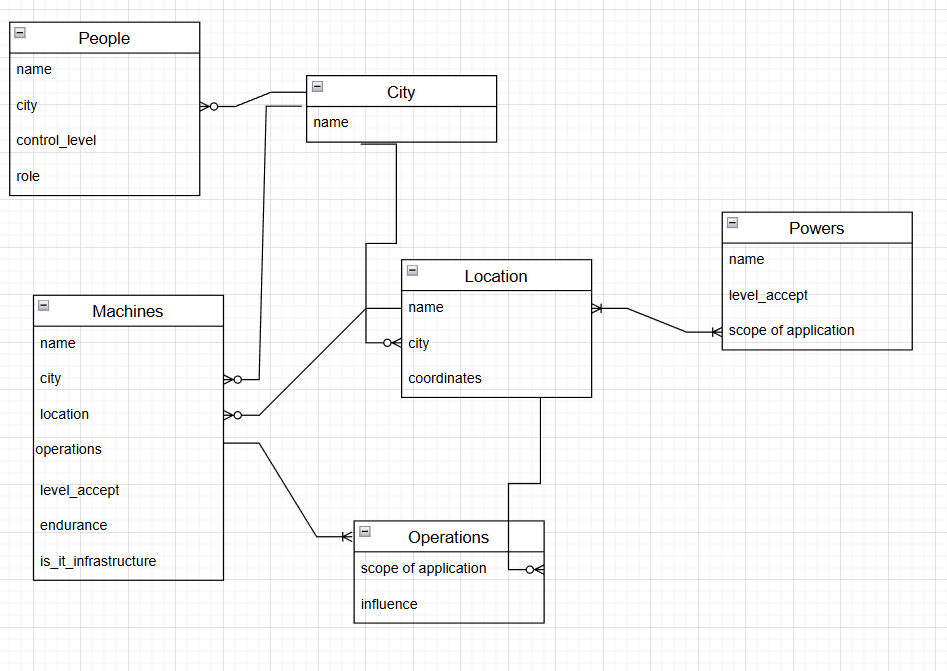
\includegraphics[scale=0.5]{images/infological.png}

\section {Даталогическая модель}
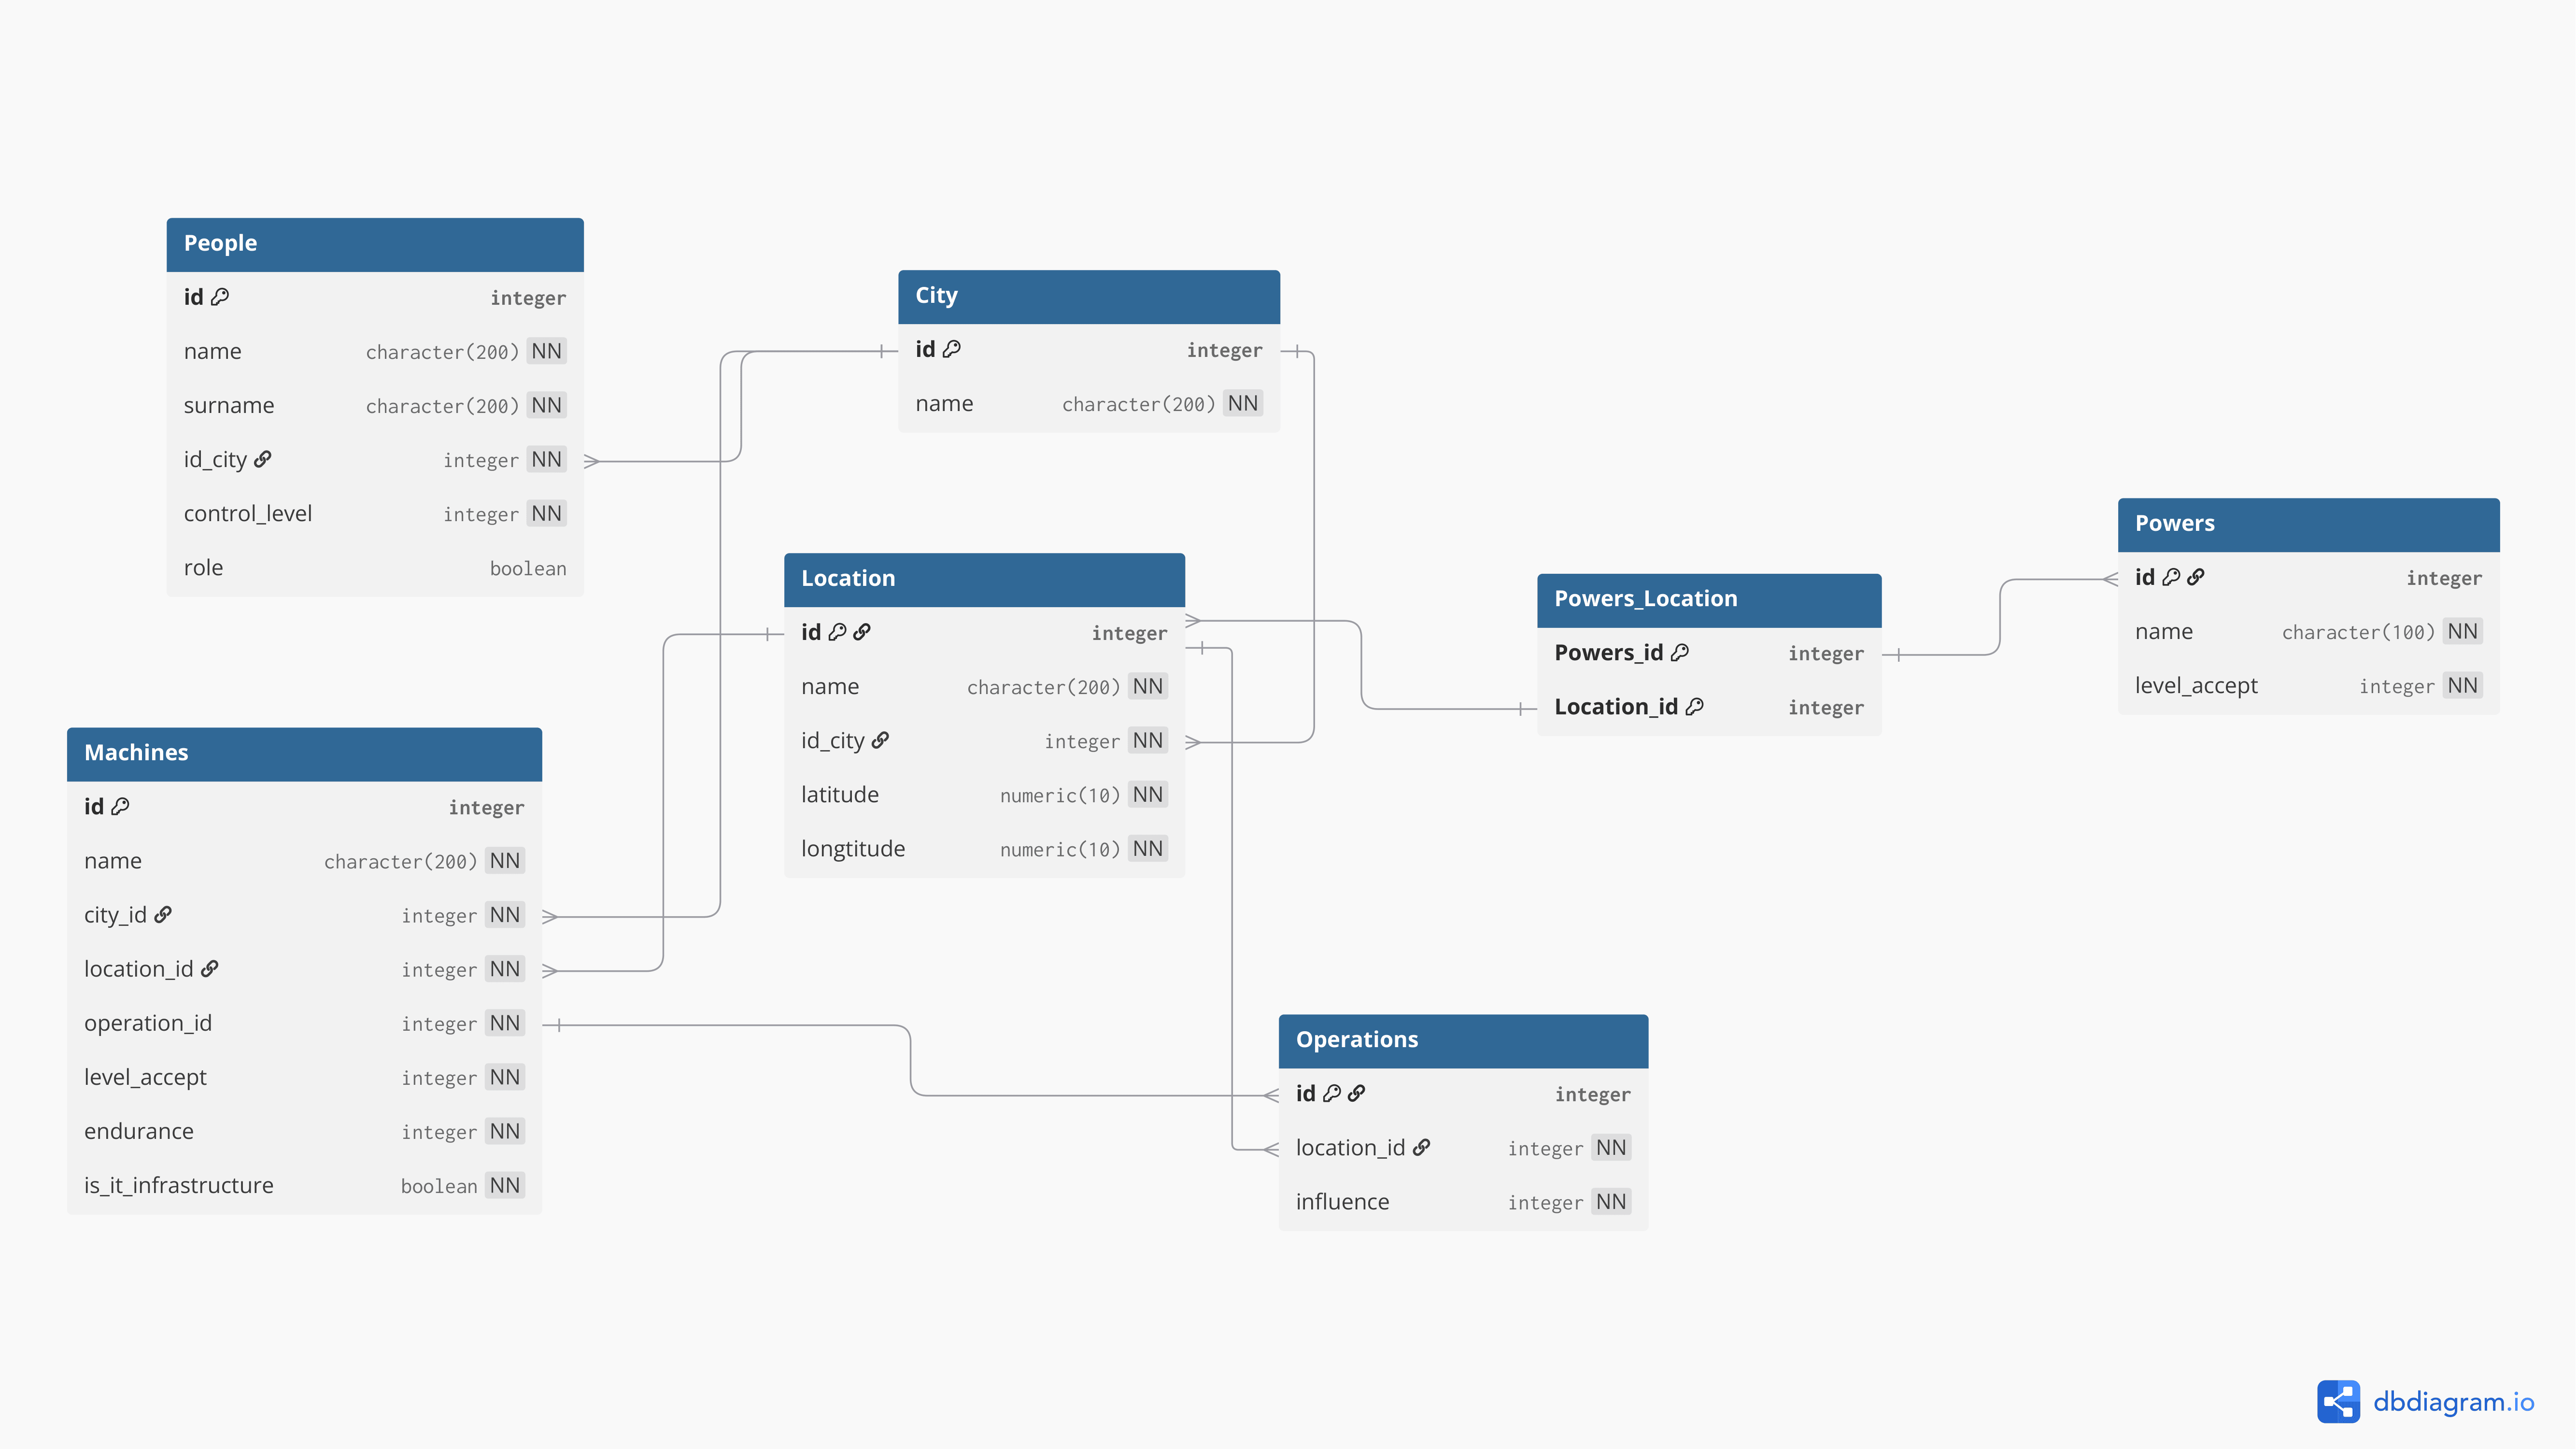
\includegraphics[scale=0.2]{images/datalogicalShema.png}
